\documentclass[11pt,oneside]{article}
\usepackage[T1]{fontenc}
\usepackage[utf8]{inputenc}
% \usepackage{lmodern}
%\usepackage[adobe-utopia,uppercase=upright,greeklowercase=upright]{mathdesign}
\usepackage[adobe-utopia]{mathdesign}
%\usepackage{minionpro}
% \usepackage{pifont}
% \usepackage{amssymb}
\usepackage{amsmath}
\usepackage[francais]{babel}
% \usepackage[francais]{varioref}
\usepackage[dvips]{graphicx}

\usepackage{framed}
\usepackage[normalem]{ulem}
\usepackage{fancyhdr}
\usepackage{titlesec}
\usepackage{vmargin}
\usepackage{longtable}

\usepackage{ifthen}


%\usepackage{epsfig}
\usepackage{subfig}

\usepackage{multirow}
\usepackage{multicol} % Portions de texte en colonnes
\usepackage{flafter}%floatants après la référence



\usepackage{color}
\usepackage{colortbl}


\definecolor{gris25}{gray}{0.75}
\definecolor{bleu}{RGB}{18,33,98}
\definecolor{bleuf}{RGB}{42,94,171}
\definecolor{bleuc}{RGB}{231,239,247}
\definecolor{rougef}{RGB}{185,18,27}
\definecolor{rougec}{RGB}{255,230,231}
\definecolor{vertf}{RGB}{103,126,82}
\definecolor{vertc}{RGB}{220,255,191}

\newenvironment{rem}[1][\hsize]%
{%
    \def\FrameCommand
    {%
\rotatebox{90}{\textit{\textsf{Remarque}}} 
        {\color{bleuf}\vrule width 3pt}%
        \hspace{0pt}%must no space.
        \fboxsep=\FrameSep\colorbox{bleuc}%
    }%
    \MakeFramed{\hsize#1\advance\hsize-\width\FrameRestore}%
}%
{\endMakeFramed}%


\newenvironment{contexte}[1][\hsize]%
{%
    \def\FrameCommand
    {%
\rotatebox{90}{\textit{\textsf{Contexte}}} 
        {\color{bleuf}\vrule width 3pt}%
        \hspace{0pt}%must no space.
        \fboxsep=\FrameSep\colorbox{bleuc}%
    }%
    \MakeFramed{\hsize#1\advance\hsize-\width\FrameRestore}%
}%
{\endMakeFramed}%

\newenvironment{savoir}[1][\hsize]%
{%
    \def\FrameCommand
    {%
\rotatebox{90}{\textit{\textsf{Savoir}}} 
        {\color{bleuf}\vrule width 3pt}%
        \hspace{0pt}%must no space.
        \fboxsep=\FrameSep\colorbox{bleuc}%
    }%
    \MakeFramed{\hsize#1\advance\hsize-\width\FrameRestore}%
}%
{\endMakeFramed}%

\newenvironment{prob}[1][\hsize]%
{%
    \def\FrameCommand%
    {%
\rotatebox{90}{\textit{\textsf{ Problématique}}} 
        {\color{rougef}\vrule width 3pt}%
        \hspace{0pt}%must no space.
        \fboxsep=\FrameSep\colorbox{rougec}%
    }%
    \MakeFramed{\hsize#1\advance\hsize-\width\FrameRestore}%
}%
{\endMakeFramed}%

\newenvironment{obj}[1][\hsize]%
{%
    \def\FrameCommand%
    {%
\rotatebox{90}{\textit{\textsf{ $\;$}}} 
        {\color{rougef}\vrule width 3pt}%
        \hspace{0pt}%must no space.
        \fboxsep=\FrameSep\colorbox{rougec}%
    }%
    \MakeFramed{\hsize#1\advance\hsize-\width\FrameRestore}%
}%
{\endMakeFramed}%

\newenvironment{defi}[1][\hsize]%
{%
    \def\FrameCommand%
    {%
\rotatebox{90}{\textit{\textsf{Définition\\}}} 
        {\color{bleuf}\vrule width 3pt}%
        \hspace{0pt}%must no space.
        \fboxsep=\FrameSep\colorbox{bleuc}%
    }%
    \MakeFramed{\hsize#1\advance\hsize-\width\FrameRestore}%
}%
{\endMakeFramed}%


\newenvironment{hypo}[1][\hsize]%
{%
    \def\FrameCommand%
    {%
\rotatebox{90}{\textit{\textsf{Hypothèse\\}}} 
        {\color{bleuf}\vrule width 3pt}%
        \hspace{0pt}%must no space.
        \fboxsep=\FrameSep\colorbox{bleuc}%
    }%
    \MakeFramed{\hsize#1\advance\hsize-\width\FrameRestore}%
}%
{\endMakeFramed}%


\newenvironment{prop}[1][\hsize]%
{%
    \def\FrameCommand%
    {%
\rotatebox{90}{\textit{\textsf{Propriété\\}}} 
        {\color{bleuf}\vrule width 3pt}%
        \hspace{0pt}%must no space.
        \fboxsep=\FrameSep\colorbox{bleuc}%
    }%
    \MakeFramed{\hsize#1\advance\hsize-\width\FrameRestore}%
}%
{\endMakeFramed}%

\newenvironment{props}[1][\hsize]%
{%
    \def\FrameCommand%
    {%
\rotatebox{90}{\textit{\textsf{Propriétés\\}}} 
        {\color{bleuf}\vrule width 3pt}%
        \hspace{0pt}%must no space.
        \fboxsep=\FrameSep\colorbox{bleuc}%
    }%
    \MakeFramed{\hsize#1\advance\hsize-\width\FrameRestore}%
}%
{\endMakeFramed}%

\newenvironment{exemple}[1][\hsize]%
{%
    \def\FrameCommand%
    {%
\rotatebox{90}{\textit{\textsf{Exemple\\}}} 
        {\color{vertf}\vrule width 3pt}%
        \hspace{0pt}%must no space.
        \fboxsep=\FrameSep\colorbox{vertc}%
    }%
    \MakeFramed{\hsize#1\advance\hsize-\width\FrameRestore}%
}%
{\endMakeFramed}%

\newenvironment{resultat}[1][\hsize]%
{%
    \def\FrameCommand%
    {%
\rotatebox{90}{\textit{\textsf{Résultat\\}}} 
        {\color{rougef}\vrule width 3pt}%
        \hspace{0pt}%must no space.
        \fboxsep=\FrameSep\colorbox{rougec}%
    }%
    \MakeFramed{\hsize#1\advance\hsize-\width\FrameRestore}%
}%
{\endMakeFramed}%

\newenvironment{methode}[1][\hsize]%
{%
    \def\FrameCommand%
    {%
\rotatebox{90}{\textit{\textsf{Méthode\\}}} 
        {\color{rougef}\vrule width 3pt}%
        \hspace{0pt}%must no space.
        \fboxsep=\FrameSep\colorbox{rougec}%
    }%
    \MakeFramed{\hsize#1\advance\hsize-\width\FrameRestore}%
}%
{\endMakeFramed}%

\newenvironment{theo}[1][\hsize]%
{%
    \def\FrameCommand%
    {%
\rotatebox{90}{\textit{\textsf{Théorème\\}}} 
        {\color{rougef}\vrule width 3pt}%
        \hspace{0pt}%must no space.
        \fboxsep=\FrameSep\colorbox{rougec}%
    }%
    \MakeFramed{\hsize#1\advance\hsize-\width\FrameRestore}%
}%
{\endMakeFramed}%

\newenvironment{warn}[1][\hsize]%
{%
    \def\FrameCommand%
    {%
\rotatebox{90}{\textit{\textsf{Attention\\}}} 
        {\color{rougef}\vrule width 3pt}%
        \hspace{0pt}%must no space.
        \fboxsep=\FrameSep\colorbox{rougec}%
    }%
    \MakeFramed{\hsize#1\advance\hsize-\width\FrameRestore}%
}%
{\endMakeFramed}%

% \usepackage{pstricks}
%\usepackage{minitoc}
% \setcounter{minitocdepth}{4}

\setcounter{tocdepth}{2}

% \mtcselectlanguage{french} 

%\usepackage{draftcopy}% "Brouillon"
% \usepackage{floatflt}
\usepackage{psfrag}
%\usepackage{listings} % Permet d'insérer du code de programmation
\renewcommand{\baselinestretch}{1.2}

% Changer la numérotation des figures :
% ------------------------------------
% \makeatletter
% \renewcommand{\thefigure}{\ifnum \c@section>\z@ \thesection.\fi
%  \@arabic\c@figure}
% \@addtoreset{figure}{section}
% \makeatother
 


%%%%%%%%%%%%
% Définition des vecteurs %
%%%%%%%%%%%%
 \newcommand{\vect}[1]{\overrightarrow{#1}}

%%%%%%%%%%%%
% Définition des torseusr %
%%%%%%%%%%%%

 \newcommand{\torseur}[1]{%
\left\{{#1}\right\}
}

\newcommand{\torseurcin}[3]{%
\left\{\mathcal{#1} \left(#2/#3 \right) \right\}
}

\newcommand{\torseurstat}[3]{%
\left\{\mathcal{#1} \left(#2\rightarrow #3 \right) \right\}
}

 \newcommand{\torseurc}[8]{%
%\left\{#1 \right\}=
\left\{
{#1}
\right\}
 = 
\left\{%
\begin{array}{cc}%
{#2} & {#5}\\%
{#3} & {#6}\\%
{#4} & {#7}\\%
\end{array}%
\right\}_{#8}%
}

 \newcommand{\torseurcol}[7]{
\left\{%
\begin{array}{cc}%
{#1} & {#4}\\%
{#2} & {#5}\\%
{#3} & {#6}\\%
\end{array}%
\right\}_{#7}%
}

 \newcommand{\torseurl}[3]{%
%\left\{\mathcal{#1}\right\}_{#2}=%
\left\{%
\begin{array}{l}%
{#1} \\%
{#2} %
\end{array}%
\right\}_{#3}%
}

 \newcommand{\vectv}[3]{%
\vect{V\left( {#1} \in {#2}/{#3}\right)}
}


\newcommand{\vectf}[2]{%
\vect{R\left( {#1} \rightarrow {#2}\right)}
}

\newcommand{\vectm}[3]{%
\vect{\mathcal{M}\left( {#1}, {#2} \rightarrow {#3}\right)}
}


 \newcommand{\vectg}[3]{%
\vect{\Gamma \left( {#1} \in {#2}/{#3}\right)}
}

 \newcommand{\vecto}[2]{%
\vect{\Omega\left( {#1}/{#2}\right)}
}
% }$$\left\{\mathcal{#1} \right\}_{#2} =%
% \left\{%
% \begin{array}{c}%
%  #3 \\%
%  #4 %
% \end{array}%
% \right\}_{#5}}

%  ------------------------------------------
% | Modification du formatage des sections : | 
%  ------------------------------------------

% Grands titres :
% ---------------

\newcommand{\titre}[1]{%
\begin{center}
      \bigskip
      \rule{\textwidth}{1pt}
      \par\vspace{0.1cm}
      
      \textbf{\large #1}
      \par\rule{\textwidth}{1pt}
    \end{center}
    \bigskip
  }

% Supprime le numéro du chapitre dans la numérotation des sections:
% -----------------------------------------------------------------
\makeatletter
\renewcommand{\thesection}{\@arabic\c@section}
\makeatother


% \titleformat{\chapter}[display]
% {\normalfont\Large\filcenter}
% {}
% {1pc}
% {\titlerule[1pt]
%   \vspace{1pc}%
%   \Huge}[\vspace{1ex}%
% \titlerule]


%%%% Chapitres Comme PY Pechard %%%%%%%%%
% numéro du chapitre
\DeclareFixedFont{\chapnumfont}{OT1}{phv}{b}{n}{80pt}
% pour le mot « Chapitre »
\DeclareFixedFont{\chapchapfont}{OT1}{phv}{m}{it}{40pt}
% pour le titre
\DeclareFixedFont{\chaptitfont}{T1}{phv}{b}{n}{25pt}

\definecolor{gris}{gray}{0.75}
\titleformat{\chapter}[display]%
	{\sffamily}%
	{\filleft\chapchapfont\color{gris}\chaptertitlename\
	\\
	\vspace{12pt}
	\chapnumfont\thechapter}%
	{16pt}%
	{\filleft\chaptitfont}%
	[\vspace{6pt}\titlerule\titlerule\titlerule]

%%%%  Fin Chapitres Comme PY Pechard %%%%%%%%%


% Section, subsection, subsubsection sans serifs :
% % ----------------------------------------------

% \makeatletter
% \renewcommand{\section}{\@startsection{section}{0}{0mm}%
% {\baselineskip}{.3\baselineskip}%
% {\normalfont\sffamily\Large\textbf}}%
% \makeatother

\makeatletter
\renewcommand{\@seccntformat}[1]{{\textcolor{bleu}{\csname
the#1\endcsname}\hspace{0.5em}}}
\makeatother

\makeatletter
\renewcommand{\section}{\@startsection{section}{1}{\z@}%
                       {-4ex \@plus -1ex \@minus -.4ex}%
                       {1ex \@plus.2ex }%
                       {\normalfont\Large\sffamily\bfseries}}%
\makeatother
 
\makeatletter
\renewcommand{\subsection}{\@startsection {subsection}{2}{\z@}
                          {-3ex \@plus -0.1ex \@minus -.4ex}%
                          {0.5ex \@plus.2ex }%
                          {\normalfont\large\sffamily\bfseries}}
\makeatother
 
\makeatletter
\renewcommand{\subsubsection}{\@startsection {subsubsection}{3}{\z@}
                          {-2ex \@plus -0.1ex \@minus -.2ex}%
                          {0.2ex \@plus.2ex }%
                          {\normalfont\large\sffamily\bfseries}}
\makeatother
 
\makeatletter             
\renewcommand{\paragraph}{\@startsection{paragraph}{4}{\z@}%
                                    {-2ex \@plus-.2ex \@minus .2ex}%
                                    {0.1ex}%               
{\normalfont\sffamily\bfseries}}
\makeatother
 
\makeatletter             
\renewcommand{\paragraph}{\@startsection{paragraph}{4}{\z@}%
                                    {-2ex \@plus-.2ex \@minus .2ex}%
                                    {0.1ex}%               
{\normalfont\sffamily\bfseries Question }}
\makeatother

\renewcommand{\theparagraph}{\arabic{paragraph}} 


\makeatletter
\renewcommand{\subparagraph}{\@startsection{subparagraph}{5}{\z@}%
                                       {-2ex \@plus-.1ex \@minus .2ex}%
                                       {0.1ex}%
				    {\normalfont\normalsize\sffamily\bfseries}}
\makeatletter
% \makeatletter
% \renewcommand{\subsection}{\@startsection{subsection}{1}{2mm}%
% {\baselineskip}{.3\baselineskip}%
% {\normalfont\sffamily\large\textbf}}%
% \makeatother
% 
% \makeatletter
% \renewcommand{\subsubsection}{\@startsection{subsubsection}{2}{4mm}%
% {\baselineskip}{.15\baselineskip}%
% {\normalfont\sffamily\large\textbf}}%
% \makeatother
% 
% \makeatletter
% \renewcommand{\paragraph}{\@startsection{paragraph}{3}{6mm}%
% {\baselineskip}{.15\baselineskip}%
% {\normalfont\sffamily\large\textbf}}%
% \makeatother
 
\setcounter{secnumdepth}{4}


%  --------
% | Marges |
%  --------


% \setmarginsrb{2.5cm}{1.5cm}{2.5cm}{2cm}{1cm}{1cm}{1cm}{1cm}
\setmarginsrb{1.5cm}{1cm}{1cm}{1.5cm}{1cm}{1cm}{1cm}{1cm}

% Changer les marges localement :
% -----------------------------
\newenvironment{changemargin}[2]{\begin{list}{}{%
\setlength{\topsep}{0pt}%
\setlength{\leftmargin}{0pt}%
\setlength{\rightmargin}{0pt}%
\setlength{\listparindent}{\parindent}%
\setlength{\itemindent}{\parindent}%
\setlength{\parsep}{0pt plus 1pt}%
\addtolength{\leftmargin}{#1}%
\addtolength{\rightmargin}{#2}%
}\item }{\end{list}}



\usepackage{pst-solides3d}
\usepackage{titletoc}
\titlecontents{chapter}[+3pc]
  {\addvspace{10pt}\sffamily\bfseries}
{\contentslabel[{\pscirclebox[fillstyle=solid,fillcolor=gray!25,
linecolor=gray!25,framesep=4pt]{\textcolor{white}{\thecontentslabel}}}]{2.5pc}}
  {}
  {\dotfill \normalfont\thecontentspage\ }

\titlecontents{section}[3pc]
  {\addvspace{2pt}\sffamily}
  {\contentslabel[\thecontentslabel]{1.8pc}}
  {}
  {\dotfill \normalfont\thecontentspage\ }

\titlecontents{subsection}[5pc]
  {\addvspace{2pt}\sffamily}
  {\contentslabel[\thecontentslabel]{1.8pc}}
  {}
  {\dotfill \normalfont\thecontentspage\ }

\titlecontents{subsubsection}[8pc]
  {\addvspace{2pt}\sffamily}
  {\contentslabel[\thecontentslabel]{3pc}}
  {}
  {\dotfill \normalfont\thecontentspage\ }
%{\;\titlerule\;\normalfont\thecontentspage\ }

\titlecontents{paragraph}[9pc]
  {\addvspace{2pt}\sffamily}
  {\contentslabel[\thecontentslabel]{3.5pc}}
  {}
  {\dotfill \normalfont\thecontentspage\ }



\usepackage[raccourcis]{FAST}
\usepackage[%
    pdftitle={Conception -- Liaisons pivot par paliers lisses},
    pdfauthor={Xavier Pessoles},
    colorlinks=true,
    linkcolor=blue,
    citecolor=magenta]{hyperref}
\usepackage{schemabloc}



% \makeatletter \let\ps@plain\ps@empty \makeatother
%% DEBUT DU DOCUMENT
%% =================
\sloppy
\hyphenpenalty 10000

\newcommand{\Pointilles}[1][3]{%
\multido{}{#1}{\makebox[\linewidth]{\dotfill}\\[\parskip]
}}


\colorlet{shadecolor}{orange!15}

\newtheorem{theorem}{Theorem}


\begin{document}


\newboolean{prof}
\setboolean{prof}{true}
%------------- En tetes et Pieds de Pages ------------
\pagestyle{fancy}
\renewcommand{\headrulewidth}{0pt}

\fancyhead{}
\fancyhead[L]{%
\noindent\noindent\begin{minipage}[c]{2.6cm}
%Lycée Rouvière PTSI

\includegraphics[width=2cm]{png/logo_ptsi.png}%
\end{minipage}
}

\fancyhead[C]{\rule{12cm}{.5pt}}

\fancyhead[R]{%
\noindent\begin{minipage}[c]{3cm}
\begin{flushright}
\footnotesize{\textit{\textsf{Sciences Industrielles\\ de l'Ingénieur}}}%
\end{flushright}
\end{minipage}
}

\renewcommand{\footrulewidth}{0.2pt}

\fancyfoot[C]{\footnotesize{\bfseries \thepage}}
\fancyfoot[L]{\footnotesize{2012 -- 2013} \\ X. \textsc{Pessoles}}
\ifthenelse{\boolean{prof}}{%
\fancyfoot[R]{\footnotesize{Cours -- CI : Conception -- P}}
}{%
\fancyfoot[R]{\footnotesize{Cours -- CI : Conception}}
}



\begin{center}
 \huge\textsc{CI 4 -- Conception : Conception des mécanismes}
\end{center}

\begin{center}
 \LARGE\textsc{Chapitre 3 -- Conception des liaisons pivots -- Utilisation des paliers lisses}
\end{center}

\vspace{.5cm}

\noindent\begin{minipage}[c]{.3\linewidth}
\begin{center}
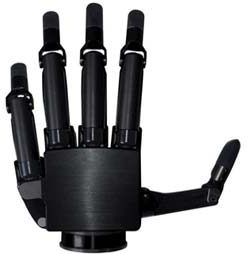
\includegraphics[height=3cm]{png/img1}

\textit{Articulations d'une prothèse de main \cite{im1}}
\end{center}
\end{minipage}\hfill
\begin{minipage}[c]{.3\linewidth}
\begin{center}
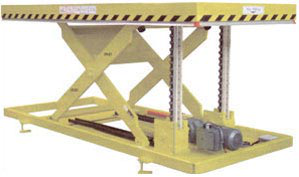
\includegraphics[height=3cm]{png/img2}

\textit{Articulations d'une table élévatrice} \cite{im2}
\end{center}
\end{minipage}\hfill
\begin{minipage}[c]{.3\linewidth}
\begin{center}
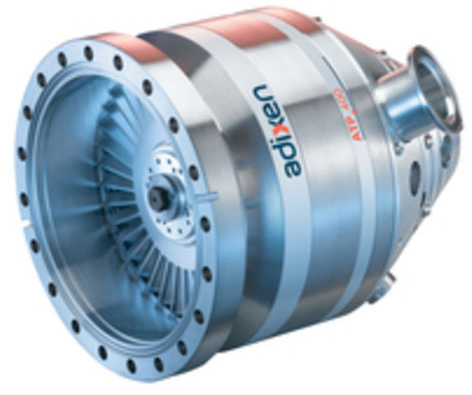
\includegraphics[height=3cm]{png/img3} 

\textit{Paliers d'une pompe turbomoléculaire} \cite{im3}\\
\end{center}
\end{minipage}

\vspace{.5cm}

Comme de nombreux systèmes en témoignent, les liaisons possédant un degré de liberté en rotation sont nombreuses dans les systèmes que nous rencontrons. Ces liaisons permettent aux solides de pivoter les uns par rapport aux aux autres, ce qui est par exemple le cas dans les moteurs, dans les réducteurs... Ces liaisons sont aussi présentes dans les systèmes articulés. 

Dans le cadre du programme de PTSI, nous nous intéressons à la conception des liaisons pivots par contact direct ou par paliers lisses. Les solutions utilisant des roulements seront abordées en PT. 

%La liaison encastrement est au c\oe{}ur de la conception des systèmes mécanique. D'une part, tous les systèmes comprennent un bâti composé de pièces fixes les unes par rapport aux autres. D'autre part, les classes d'équivalences cinématiques participant à la transmission ou à la transformation de puissance, sont elles-mêmes constituées de pièces fixes les unes par rapport aux autres. 
%
%Ces liaisons encastrement peuvent être démontables, permettant ainsi d'assurer la maintenance d'une pièce ou d'une autre. Elles peuvent être aussi permanentes (ou non démontables). Dans ce cas, il faut faire appel à des procédés d'assemblage plus ou moins difficiles à mettre en \oe{}uvre. 
%
%Parmi la multitude de solutions technologiques qui peuvent se présenter, il s'agit de choisir de façon méthodique celle à même de répondre au cahier des charges. Il s'agit ensuite de savoir la représenter en vu de concevoir un mécanisme.

\begin{prob}
\textsc{Problématique :}
\begin{itemize}
\item Comment décrire une solution pivot existante ?
\item Comment concevoir une architecture de liaison pivot ?
\item Comment dimensionner une liaison pivot ?
\item Quels éléments technologiques utiliser ?
\end{itemize}
\end{prob}

\begin{savoir}
\textsc{Savoirs :}
\begin{itemize}
\item Identifier les architectures des guidages en rotation 
\item Définir et caractériser les fonctions techniques
\item Définir les principes de réalisations
\item Définir les principales solutions de guidage en rotation avec glissement
\end{itemize}
\end{savoir}

\newpage 

\setlength{\parskip}{0ex plus 0.2ex minus 0ex}
 \renewcommand{\contentsname}{}
 \renewcommand{\baselinestretch}{1}

\tableofcontents

 \renewcommand{\baselinestretch}{1.2}
\setlength{\parskip}{2ex plus 0.5ex minus 0.2ex}

% \vspace{1cm}
\textit{Ce document est en évolution permanente. Merci de signaler toutes
erreurs ou coquilles.}


\section{Cahier des charges d'une liaison pivot}

Le cahier des charges d'une liaison pivot peut se présenter ainsi :


%
%\noindent\begin{minipage}[t]{.23\linewidth}
%\noindent\colorbox{gris25}{\makebox[\textwidth][l]{%
%\textbf{\textsf{\textcolor{black}{Méthode statique}}}
%}}
%\end{minipage}\hfill
%\begin{minipage}[t]{.23\linewidth}
%
%\end{minipage}\hfill
%\begin{minipage}[t]{.23\linewidth}
%
%\end{minipage}\hfill
%\begin{minipage}[t]{.23\linewidth}
%
%\end{minipage}



\begin{center}
\begin{tabular}{|p{.2\textwidth}|p{.2\textwidth}|p{.2\textwidth}|p{.2\textwidth}|}
\hline
\textbf{Fonctions} & \textbf{Critères} & \textbf{Niveau} & \textbf{Flexibilité} \\
\hline
Positionner les deux pièces entre elles & Précision du guidage, (isostatisme, critère L/D)	& Tx, Ty, Tz (en mm)
Ry, Rz (en rad)	maxi  &\\
\hline
Guider, permettre un mouvement relatif de rotation & 
Rendement & $\eta$  en \% mini &\\
\cline{2-4}
& Vitesse de rotation & $\omega$  (en rad/s) & \% \\
\hline
Transmettre et supporter les efforts & Efforts transmissibles	& X, Y, Z (en N) M, N (en Nm) & \% \\
& Durée de vie & Temps (h) & maxi \\
\cline{2-4}
Résister à l'ambiance extérieure	& Température, humidité, poussière & & \\
\hline
\end{tabular}
\end{center}

D'autres fonctions de service peuvent également être mises en évidence : 
\begin{itemize}
\item préserver l'environnement : bruit, pollution;
\item permettre le montage / la maintenance : temps et facilité de montage;
\item s'intégrer dans le mécanisme : encombrement.
\end{itemize}

\section{Les solutions techniques}


\FASTInterligne=.2cm %Nouvel interligne
\begin{FAST}{Guider 2 pièces en rotation}
\FASTFT{FP1 -- Réaliser un contact glissant entre 2 surfaces}{%
	\FASTFT{FP11 -- Réaliser un contact direct}{%
		\FASTST{Cylindre et butée}
		\FASTDecalageOuHorizontal=0pt
		\FASTST[ou]{Cylindre court et plan}
	%\FASTDecalageOuHorizontal=0pt
		%\FASTST[ou]{Cône (pivot)}
		}
	\FASTFT{FP12 -- Utiliser un matériau antifriction}{
		\FASTST{Bagues lisses}
		\FASTDecalageOuHorizontal=0pt
		\FASTST[ou]{Bagues à collerette}
		\FASTDecalageOuHorizontal=0pt
		\FASTST[ou]{Rotules lisses}
}}
\FASTFT{FP2 -- Interposer des éléments roulants}{ 
\FASTFT{FP21 -- Interposer des billes}{%
		\FASTST{Rigides 1 rangée}
		\FASTDecalageOuHorizontal=0pt
		\FASTST[ou]{Rigides 2 rangées}
	       \FASTDecalageOuHorizontal=0pt
		\FASTST[ou]{Contacts obliques}
	       \FASTDecalageOuHorizontal=0pt
		\FASTST[ou]{Rotules}
		}
\FASTFT{FP22 -- Interposer des rouleaux coniques}{%
		\FASTST{Une rangée}
	       \FASTDecalageOuHorizontal=0pt
		\FASTST[ou]{Deux rangées}
               }
\FASTFT{FP23 -- Interposer des rouleaux cylindriques}{%
		\FASTST{Sans épaulement}
	       \FASTDecalageOuHorizontal=0pt
		\FASTST[ou]{Avec épaulement}
               }
\FASTFT{FP24 -- Interposer des aiguilles}{%
		\FASTST{Simples}
	       \FASTDecalageOuHorizontal=0pt
		\FASTST[ou]{Combinés}
               }
}
\FASTFT{FP3 -- Séparer les surfaces}{
\FASTFT{FP31 -- Générer la pression}{%
		\FASTST{Paliers hydrostatiques}
               }
\FASTFT{FP32 -- Générer des effets hydrodynamiques}{%
		\FASTST{Paliers hydrodynamiques}
               }
\FASTFT{FP33 -- Réaliser une sustentation électromagnétique}{%
		\FASTST{Paliers magnétiques actifs}
}}
\end{FAST}
\FASTReset %Remise à zéro


\subsection{Satisfaire la fonction « Positionner» : isostatisme}
Le positionnement sera d'autant plus précis que le montage sera isostatique.

Pour assurer une liaison pivot, on trouve globalement l'association des liaisons suivantes : 
\begin{itemize}
\item pivot glissant et sphère --plan;
\item appui plan et sphère--cylindre;
\item rotule et sphère--cylindre.
\end{itemize}

Pour assurer une liaison pivot glissant, on peut trouver les solutions suivantes : 
\vspace{.5cm}

\noindent\begin{minipage}[c]{.43\linewidth}
\begin{center}
Deux centrages courts

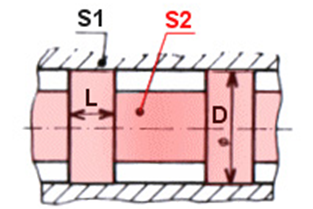
\includegraphics[width=.5\textwidth]{png/fig02}

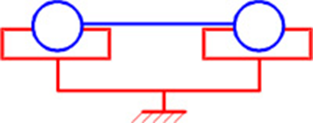
\includegraphics[width=.5\textwidth]{png/fig03}
\end{center}
\end{minipage}\hfill
\begin{minipage}[c]{.43\linewidth}
\begin{center}
Un centrage long

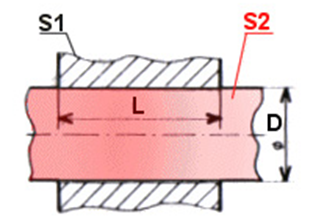
\includegraphics[width=.5\textwidth]{png/fig04}

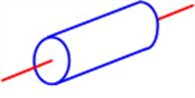
\includegraphics[width=.5\textwidth]{png/fig05}

\end{center}
\end{minipage} 
\subsection{Satisfaire la fonction « Guider» : rendement}
Le guidage doit se faire en limitant les pertes par frottement. Selon les conditions d'utilisation (vitesse, effort), les solutions peuvent être soit par glissement, soit par roulement.


\noindent\begin{minipage}[t]{.23\linewidth}
\begin{center}
Contact direct
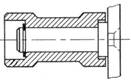
\includegraphics[width=.9\textwidth]{png/fig06}
\end{center}
\end{minipage}\hfill
\begin{minipage}[t]{.23\linewidth}
\begin{center}
Interposition de bagues
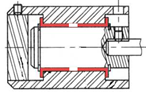
\includegraphics[width=.9\textwidth]{png/fig07}
\end{center}
\end{minipage}\hfill
\begin{minipage}[t]{.23\linewidth}
\begin{center}
Interposition de fluide
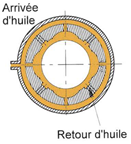
\includegraphics[width=.9\textwidth]{png/fig08}
\end{center}
\end{minipage}\hfill
\begin{minipage}[t]{.23\linewidth}
\begin{center}
Interposition d'éléments roulants
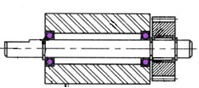
\includegraphics[width=.9\textwidth]{png/fig09}
\end{center}
\end{minipage}


\begin{center}
\begin{tabular}{|p{.3\textwidth}|p{.2\textwidth}|p{.2\textwidth}|p{.2\textwidth}|}
\hline
\multirow{2}*{\textbf{Type de guidage en rotation}} & \multicolumn{3}{|c|}{\textbf{Contraintes}}\\
\cline{2-4}
& Précision & Vitesse de rotation & Efforts à transmettre \\
\hline
Par contact direct & - & - - & - \\
\hline
Par interposition de bague de frottement & + & + & + \\
\hline
Par interposition d'éléments roulants & ++ & ++ & +++ \\
\hline 
Par interposition d'un film lubrifiant & +++ & +++ & ++ \\
\hline
\end{tabular}
\end{center}

%\begin{center}
%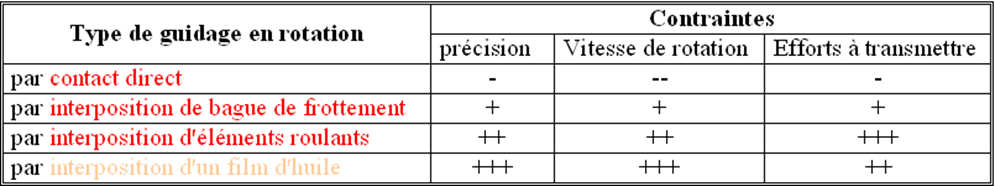
\includegraphics[width=.9\textwidth]{png/fig10}
%\end{center}  
%FAST
									
\subsection{Satisfaire la fonction « transmettre les efforts» : dimensionnement}

Le dimensionnement de chacune des solutions précédentes dépend des types de solutions mais les principaux critères communs sont : 
\begin{itemize}
\item la vitesse périphérique;
\item les efforts à transmettre ou la pression de contact;
\item les conditions environnantes (poussière, milieux corrosifs…);
\item la durée de vie souhaitée.
\end{itemize}

\section{Guidage par interposition de bagues}

Économiques, souvent utilisés, les coussinets sont des bagues cylindriques, de forme tubulaire, avec ou sans collerette, interposés entre un arbre et son logement pour faciliter le mouvement de rotation en limitant les pertes par frottement.

Construits à partir de matériaux présentant de bonnes qualités frottantes (bronze, étain, plomb, graphite, Téflon, PTFE, polyamide), ils peuvent être utilisés à sec ou avec lubrification.

\subsection{Les différents types}
On distingue les paliers avec contact, et les paliers sans contact. Les premiers présentent évidemment davantage de frottements.

\subsubsection{Coussinets autolubrifiants}
Ils sont fabriqués à partir de métal fritté\footnote{Frittage : procédé de mise en forme des poudres. De la poudre est chauffée dans un moule, en dessous de la température de fusion. La poudre va se souder pour donner une pièce solide. } à base de bronze (\textbf{$Cu\,Sn\,8$}). 

Le frittage permet d'obtenir des pièces poreuses (porosités entre 15 et 35\% en volume) et ainsi d'y incorporer du lubrifiant (huile, graphite...). Dans le cas de l'huile, la structure, comparable à une éponge, restitue l'huile en fonctionnement et l'absorbe à l'arrêt. 
 		 

\noindent\begin{minipage}[c]{.23\linewidth}
\begin{center}
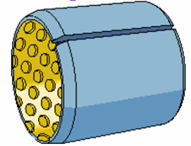
\includegraphics[width=.75\textwidth]{png/fig11}
\end{center}
\end{minipage}\hfill
\begin{minipage}[c]{.23\linewidth}
\begin{center}
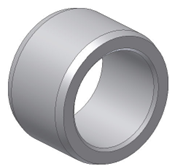
\includegraphics[width=.75\textwidth]{png/fig12}
\end{center}
\end{minipage}\hfill
\begin{minipage}[c]{.23\linewidth}
\begin{center}
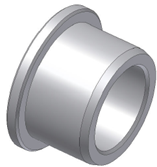
\includegraphics[width=.75\textwidth]{png/fig13}
\end{center}
\end{minipage}\hfill
\begin{minipage}[c]{.23\linewidth}
\begin{center}
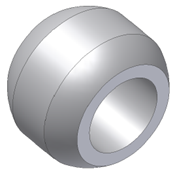
\includegraphics[width=.75\textwidth]{png/fig14}
\end{center}
\end{minipage}

		 
\subsubsection{Les coussinets composites type "glacier"}

\begin{minipage}[c]{.7\linewidth}
La base est une tôle d'acier roulée recouverte d'une couche de bronze fritté. La surface frottante peut être en résine acétal ou en PTFE avec addition d'un lubrifiant solide : plomb, graphite, bisulfure de molybdène $MoS_2$...
Ils peuvent fonctionner à sec ou avec un léger graissage au montage sous des vitesses périphériques inférieures à $3\; m/s$. 
\end{minipage}\hfill
\begin{minipage}[c]{.25\linewidth}
\begin{center}
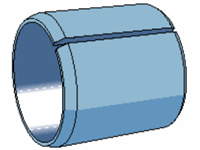
\includegraphics[width=.75\textwidth]{png/fig15}
\end{center}
\end{minipage}

\subsubsection{Les coussinets polymères (Nylon, PTFE, acétal...)}
\begin{minipage}[c]{.7\linewidth}
Surtout utilisés lorsqu'il est nécessaire d'avoir une grande résistance chimique (acides, bases, éléments corrosifs...) et une grande légèreté.
Inconvénients : le fluage\footnote{Déformation permanente d'un matériau sous l'effet d'une contrainte inférieure à la la résistance élastique ($Re$).} sous charge et un faible coefficient de conductivité thermique empêchant une bonne évacuation des calories.
\end{minipage}\hfill
\begin{minipage}[c]{.25\linewidth}
\begin{center}
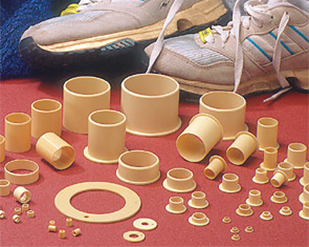
\includegraphics[width=.75\textwidth]{png/fig16}
\end{center}
\end{minipage}

%Les Paliers Lisses Polymères ont par exemple été utilisés pour la fourche « Magura Durin Race » du vélo olympique. Il a été réalisé en « iglidur J » afin de réduire son poids. Les Paliers Lisses Polymères réalisés dans ce matériau sont parfaits pour l'application en question, qui exige une extrême résistance à l'usure ainsi qu'une grande réactivité. Ces Paliers Lisses Polymères sont environ cinq fois plus légers que des paliers métalliques de mêmes cote

\subsubsection{Rotules lisses}
Elles permettent de corriger les défauts d'alignement. 
\begin{center}
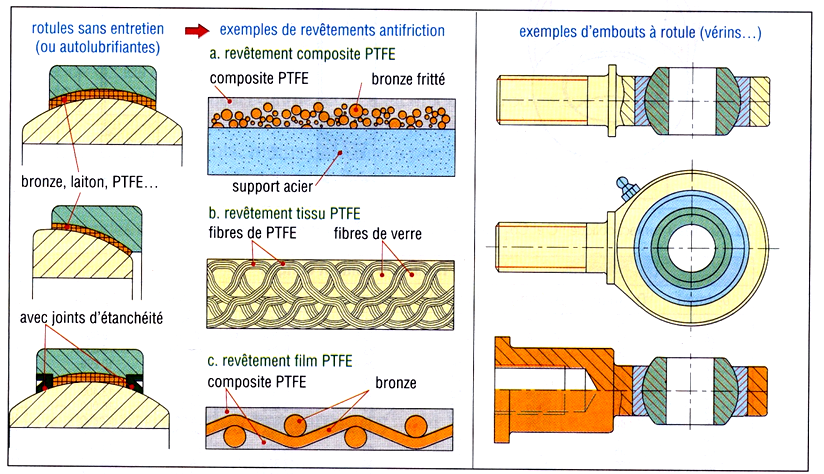
\includegraphics[width=.75\textwidth]{png/fig17}
\end{center}

%\subsubsection{Synthèse des performances}
%
%\begin{center}
%\begin{tabular}{|p{4cm}|p{4cm}|p{4cm}|p{4cm}|}
%\cline{2-4}
%\multicolumn{1}{c|}{} & Coussinets autolubrifiants& Coussinets type glacier & Coussinets polymères\\
%\hline 
%Vitesse circonférentielle maximale ($m/s$) & 
%\begin{itemize}
%\item $13\; m/s$ (carbone, graphite) 
%\item 7 à 8 $m/s$ 
%\end{itemize}& 
%2 à 3 $m/s$ & 
%2 à 3 $m/s$ \\
%\hline
%Températures limites de fonctionnement (degrés C) & 
%\begin{itemize}
%\item jusqu'à 400\degre C (graphite)
%\item jusqu'à 250\degre C (bronze -- plomb) 
%\end{itemize}&
%\begin{itemize}
%\item -40\degre C à + 110 \degre C (acétal) 
%\item -200\degre C à + 280 \degre C (PTFE)
%\end{itemize} &
%\begin{itemize}
%\item -40\degre C à + 100 \degre C (acétal) 
%\item -80\degre C à + 120 \degre C (Nylon) 
%\end{itemize}
%\\
%\hline
%Pression diamétrale admissible $p$ ($N/mm^2$) &
%\begin{itemize}
%\item 5 $N/mm^2$ (graphite)
%\item 20 à 30 $N/mm^2$ (bronze -- plomb)
%\item 7 à 35 $N/mm^2$ (bronze -- étain) 
%\end{itemize}&
%\begin{itemize}
%\item 70 $N/mm^2$ (acétal)
%\item 50 $N/mm^2$ (PTFE) 
%\end{itemize}&
%7 à 10 $N/mm^2$ 
%\\
%\hline
%Produit $p\cdot V$
%($N/mm^2 \times m/s$) &
%\begin{itemize}
%\item 0,5 graphite
%\item 1,8 à 2,8 (bronze -- plomb)
%\item 1,7 (bronze -- étain) 
%\end{itemize}&
%\begin{itemize}
%\item 3 (acétal) 
%\item 1,8 à 3,6 (PTFE)
%\end{itemize} &
%\begin{itemize}
%\item 0,1 (acétal)
%\item 0,1 à 0,42 (Nylon) 
%\end{itemize}\\
%\hline
%\end{tabular}
%\end{center}

\subsection{Montage}
\subsubsection{Architecture}
\paragraph*{Surface(s) assurant le pivot glissant :}
Un centrage long (cylindre long) ou deux centrages courts (cylindre court)
\paragraph*{Surface(s) assurant la butée :}
Pour assurer la bilatéralité du contact, il faut deux plans parallèles ("petits"), et donc un jeu axial minimal pour garantir la rotation sans coincement sous l'effet des défauts de fabrication et des variations de longueur dues aux dilatations 

\begin{center}
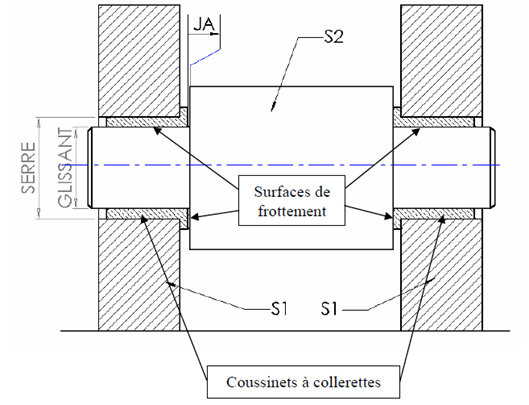
\includegraphics[width=.75\textwidth]{png/fig19}
\end{center}

\subsubsection{Contraintes à imposer aux surfaces d'accueil}
\paragraph*{Ajustement}
La précision du guidage (jeu angulaire limité) limite le jeu diamétral entre l'arbre et le coussinet  à 2 à 4/1000 du diamètre.

\begin{center}
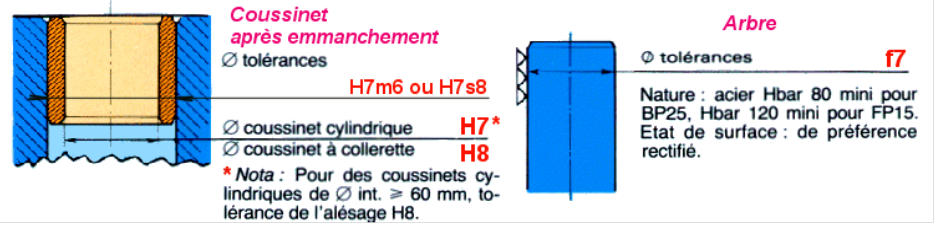
\includegraphics[width=.9\textwidth]{png/fig18}
\end{center}
 
Sur le dessin d'ensemble on se contente de faire figurer les ajustements, 
\begin{itemize}
\item dans la zone de glissement : f7 
\item et dans la zone d'encastrement des bagues : H7 pour l'alésage de fixation (la dimension de la bague avant montage est souvent s7 pour qu'après son montage dans un alésage H7, l'alésage de la bague soit H7).
\end{itemize}

\begin{itemize}
\item Jeu axial :
\begin{itemize}
\item Le jeu axial sera indiqué sous la forme d'une condition fonctionnelle.
\end{itemize}
\item État de surface :
\begin{itemize}
\item on impose une rugosité conforme aux préconisations du constructeur : $Ra\, 0,8\; \text{maxi}$
\end{itemize}
\item Dureté de l'arbre
\begin{itemize}
\item une portée de glissement de l'arbre durcie superficiellement (écrouissage ou trempe) donne de meilleurs résultats (moins de risque de grippage).
\end{itemize}
\end{itemize}

\paragraph*{Contraintes géométriques :}
Les surfaces accueillant les coussinets doivent porter une tolérance de cylindricité. 

Lorsque deux paliers lisses sont nécessaires pour réaliser la liaison pivot, une spécification de coaxialité doit être portée entre les axes des alésages. 

Enfin, pour les paliers à collerettes, une spécification de perpendicularité peut être portée
entre l'axe du  cylindre et le plan d'appui.

\subsection{Dimensionnement : critères de choix}
La procédure de calcul varie sensiblement d'une famille à l'autre et d'un fabricant à l'autre. Pour des choix précis utiliser les documents constructeurs. Cependant ces calculs (durée de vie, longueur du coussinet...) font régulièrement intervenir les notions de pression diamétrale P et de produit PV.

\subsubsection{Pression}
Pour éviter les phénomènes de matage, on impose un critère de pression admissible maximal.
On applique le critère de la pression diamétrale moyenne et on vérifie que la valeur reste inférieure au maximum possible pour le cas étudié.
Cette pression diamétrale est déterminée en supposant que la répartition de pression est uniforme et répartie sur un demi-cylindre. 


\begin{center}
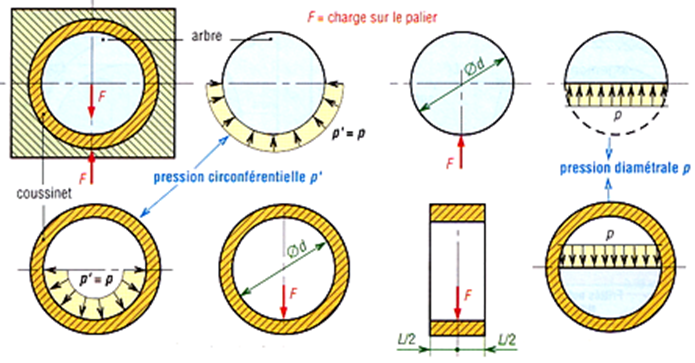
\includegraphics[width=.75\textwidth]{png/fig20}
\end{center}

Pression diamétrale :
\begin{center}
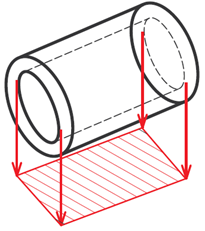
\includegraphics[width=.3\textwidth]{png/fig21}
\end{center}
$$ 
p=\dfrac{F}{L\cdot d} < p_{adm}
$$

\begin{exemple}
Rappel de la démonstration de l'effort engendré par une pression constante :

\rotatebox{90}{
\begin{tabular}{p{10cm}}
 \\
\end{tabular}}
\end{exemple}
\subsubsection{Vitesse}

Le paramètre important est la vitesse linéaire au niveau du contact coussinet/arbre. Cette vitesse doit etre limitée pour éviter une usure trop importante : $\vectv{M}{\text{arbre}}{\text{coussinet}}  =R_{\text{arbre}}\cdot  \omega_{arbre/bati}<V_{\text{limite}}$ (m/s).
On doit aussi vérifier que cette vitesse ne dépasse celle qui est préconisée par le constructeur.

\subsubsection{Produit PV}
\noindent\begin{minipage}[c]{.45\linewidth}
Il existe des combinaisons pression/vitesse pour lesquelles le palier s'échauffe trop : la température du palier augmente et la destruction est rapide
Le produit pV, caractérise l'énergie dissipée dans le palier par unité de surface. 
Il est donc caractéristique de la chaleur dégagée dans la zone de contact, donc de l'usure et du risque de grippage. 
\end{minipage}\hfill
\begin{minipage}[c]{.45\linewidth}

\begin{center}
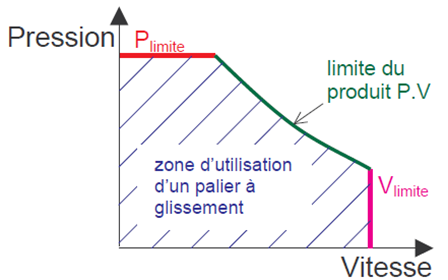
\includegraphics[width=.9\textwidth]{png/fig22}
\end{center}
\end{minipage}
Les fabricants de bagues standard donnent des valeurs  admissibles en fonction des conditions d'utilisation et des matériaux constituant les bagues.
\subsubsection{Frottement}
\noindent\begin{minipage}[c]{.45\linewidth}
\begin{center}
Frottement sur la surface cylindrique
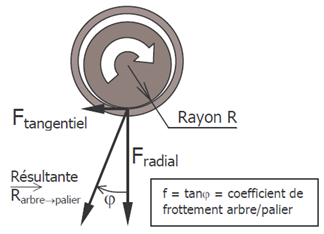
\includegraphics[height=3cm]{png/fig23}
\end{center}
On a : 
$$
C_f = \tan \varphi F_{Radial}\cdot R
$$ 
\end{minipage}\hfill
\begin{minipage}[c]{.45\linewidth}
\begin{center}
Frottement sur l'épaulement

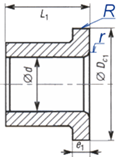
\includegraphics[height=3cm]{png/fig24}
En cas d'utilisation de coussinets à collerettes, il faut ajouter le couple de frottement de l'arbre contre l'épaulement
$$
C_f = \dfrac{2}{3}\dfrac{fN\left( R^3-r^3\right)}{\left( R^2-r^2\right)}
$$
\end{center}
\end{minipage}

 
 

On peut alors déterminer la puissance perdue par frottement : $P = C_f \cdot \omega $
\begin{itemize}
\item $P$: puissance dissipée exprimée en Watt (W)
\item $C_f$: couple de frottements (N.m)
\item $\omega$ : vitesse angulaire de l'arbre par rapport au bati (en rad/s)
\end{itemize}

Cette puissance correspond à l'énergie qu'il faut évacuer pour chaque unité de temps sous forme de chaleur. La chaleur s'évacue: 
\begin{itemize}
\item par le bâti : Surface d'échange importante, faible élévation de la température. 
\item par l'arbre: Surface d'échange limitée, élévation de la température. 
\end{itemize}

Cette élévation de la température modifie: 
\begin{itemize}
\item les jeux de fonctionnement par dilatation (risque de grippage pour jeu initial insuffisant);
\item les qualités du lubrifiant;
\item les caractéristiques physiques des matériaux. 
\end{itemize}

\subsection{Protection}
Les paliers sont généralement peu sensibles aux impuretés. Lorsque l'environnement est pollué, on peut avoir recourt aux solutions suivantes : 
 

\noindent\begin{minipage}[c]{.3\linewidth}
\begin{center}
Protection par les éléments voisins
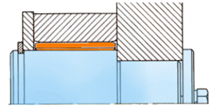
\includegraphics[width=.85\textwidth]{png/fig25}
\end{center}
\end{minipage}\hfill
\begin{minipage}[c]{.3\linewidth}
\begin{center}
Joint à lèvre
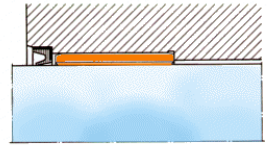
\includegraphics[width=.85\textwidth]{png/fig26}
\end{center}
\end{minipage}\hfill
\begin{minipage}[c]{.3\linewidth}
Joint spéciaux
\begin{center}
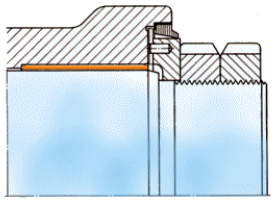
\includegraphics[width=.9\textwidth]{png/fig27}
\end{center}
\end{minipage}
 
 
		
\subsection{Comparaison}
\begin{center}
\begin{tabular}{|p{.17\textwidth}|p{.17\textwidth}|p{.17\textwidth}|p{.17\textwidth}|p{.17\textwidth}|}
\hline
\multicolumn{5}{|c|}{\textbf{Performances comparatives des coussinets usuels}}\\
\hline
Type de coussinet 
& Vitesse maximale admissible $(m/s)$ 
& Températures limites de fonctionnement $(^oC)$ 
& Pression admissible en fonctionnement $(MPa)$
& Produits PV admissibles $(MPa\cdot m/s)$ \\
\hline
Glacier acétal & 2 à 3 & -40 à 100 & 14 & 0,5 à 0,9 \\
\hline
Glacier PTFE & 3 & -200 à 280 & 20 & 0,9 à 1,5 \\
\hline
Graphite & 13 & 400 & 5 & 0,5 \\
\hline
Bronze -- étain & 7 à 8 & >250 & 7 à 35 & 1,7 \\
\hline
Bronze -- plomb & 7 à 8 & 250 & 20 à 30 & 1,8 à 2,1 \\
\hline
Nylon & 2 à 3 & -80 à 120 & 7 à 10 & 0,1 à 0,3 \\
\hline
Acétal & 2 à 3 & -40 à 100 & 7 à 10 & 0,1 \\
\hline
\end{tabular}
\end{center}
%\begin{center}
%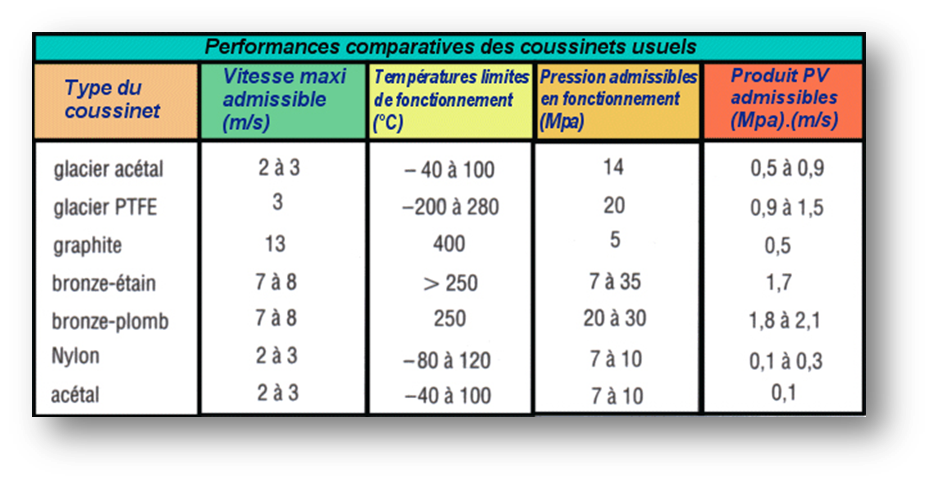
\includegraphics[width=.9\textwidth]{png/fig28}
%\end{center} 

\section{Guidage sans contact solide}
\subsection{Paliers hydrodynamique et hydrostatique}

Ils  peuvent tourner plus vite et plus longtemps…Les paliers hydrostatiques sont bien adaptés au cas de charges importantes.
Application : broches d'aléseuses et de rectifieuses de grande précision, rotor de la pompe primaire des réacteurs nucléaires N4


\noindent\begin{minipage}[c]{.55\linewidth}
\begin{center}
Palier hydrodynamique

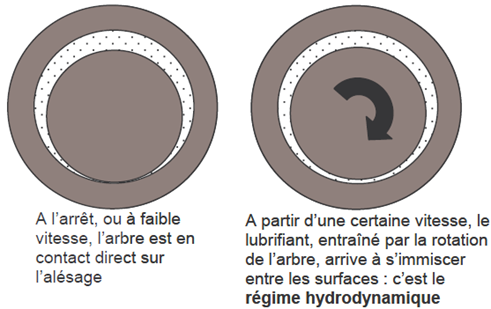
\includegraphics[width=.6\textwidth]{png/fig29}
\end{center}
Avantage : économique par rapport à ceux de droite
Inconvénient : surfaces mal lubrifiées au démarrage	
\end{minipage}\hfill
\begin{minipage}[c]{.35\linewidth}
\begin{center}
Palier hydrostatique
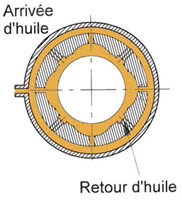
\includegraphics[width=.6\textwidth]{png/fig30}
\end{center}
Avantage : charges importantes, peu de pertes
Inconvénient : couteux, nécessite une pompe
\end{minipage}

	
 	

\subsection{Paliers magnétiques}

Développés à l'origine pour des besoins militaires et spatiaux, les paliers à sustentation magnétique prennent leur essor industriel dans les machines tournantes et les pompes à vide.
Son rotor « flotte » dans un champ de forces électromagnétiques contrôlées, donc sans contact, sans frottement, sans pertes d'énergie, sans lubrifiant.


\noindent\begin{minipage}[c]{.55\linewidth}
\begin{center}
Palier magnétique

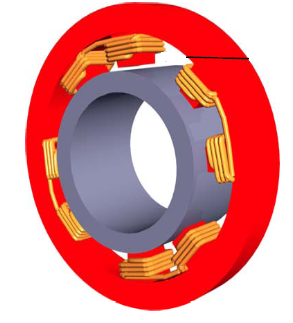
\includegraphics[height=3.5cm]{png/fig31}
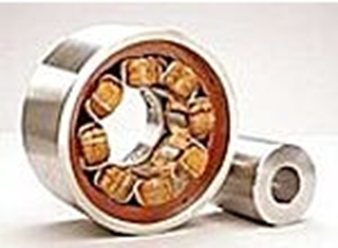
\includegraphics[height=3.5cm]{png/fig32}
\end{center}
\end{minipage}\hfill
\begin{minipage}[c]{.4\linewidth}
\begin{center}
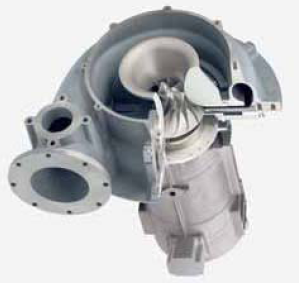
\includegraphics[height=3.5cm]{png/fig33}
\end{center}
\end{minipage}

    
 
Applications : Machines rapides motorisées :

\begin{center}
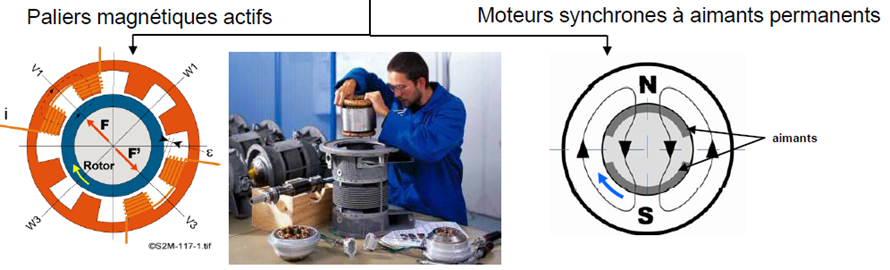
\includegraphics[width=.9\textwidth]{png/fig34}
\end{center}

\begin{itemize}
\item pas de lubrification nécessaire, pas de pollution du process;
\item très grande vitesse périphérique possible (jusqu'à 250 m/s);
\item très faible niveau de vibrations (contrôle dynamique);
\item pertes faibles;
\item très bon rendement;
\item faible allongement du rotor.
\end{itemize}
Exemple : Microturbine à gaz pour la production d'électricité et d'eau chaude
  
\begin{minipage}[c]{.4\textwidth}
\begin{center}
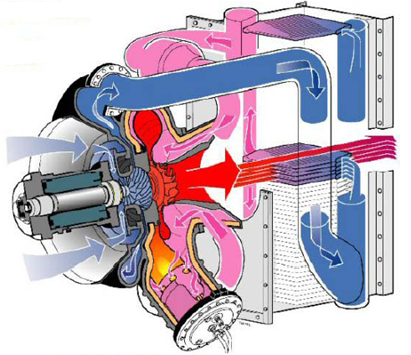
\includegraphics[width=.9\textwidth]{png/fig35}
\end{center}
\end{minipage}\hfill
\begin{minipage}[c]{.4\textwidth}
\begin{center}
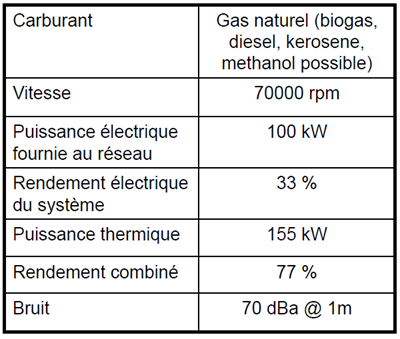
\includegraphics[height=4cm]{png/fig36}
\end{center}
\end{minipage}

Autres exemple : Guidages sur les machines outils d'UGV 



\begin{thebibliography}{2}
\bibitem{im1}{\url{http://www.igus.fr/wpck/default.aspx?Pagename=Manus11_Handprothese&CL=DE-en}}
\bibitem{im2}{\url{http://www.igus.fr/wpck/default.aspx?Pagename=app_actuatingmechanism&CL=FR-fr}}
\bibitem{im3}{\url{http://www.usinenouvelle.com/expo/img/pompes-turbomoleculair-000111712-4.jpg}}
\bibitem{mc}{Conception -- Guidage en rotation -- Guidage par paliers lisses, Supports de cours de Maryline Carrez, Lycée Jules Haag, Besançon}
\bibitem{LP}{Construction Mécanique -- Les paliers lisses ou coussinets -- Familles de coussinets, dimensionnement, montage, comparatif, Didier Noël ??, LP Pierre et Marie Curie, Aulnoye \url{http://noel.wifeo.com/documents/Les-Paliers-lisses-ou-Coussinets.pdf}}
\end{thebibliography}

\end{document}